% !TEX root = ../double_trouble_main.tex

We next show that our method performs well on a real dataset in cancer genomics and semi-synthetic dataset in population genetics. We confirm that our method performs better than the independent and dependent applications of one-population methods.

\paragraph{Comparisons.} For the real datasets, we find that different one-population methods exhibit substantially different performance for different types of data. So, for each type of data (cancer, population genetics), we test a variety of different one-population methods. In Section S7.2 of the Supplementary Material \citep{supplement}, we compare them on the one-population task and choose the best-performing method to serve as the comparison (via independent and dependent applications) for our two-population method. \internal{In particular, we choose the one-population method with the lowest root mean squared error of the prediction curve for the number of variants; here, we take the mean across all values of the follow-up sample size (up to the largest value), and we note that this value depends on our choice of ordering of the data points.} For one-population methods, we consider the fourth-order jackknife \citep{burnham1978estimation, gravel2014predicting}, the Good-Toulmin estimator \citep{Orlitsky2016,chakraborty2019using}, linear programming \citep{zou2016quantifying}, the 3BP approach of \citet{Masoero2022}, and the scaled process of \citet{Camerlenghi2021}.


\paragraph{Two cancer genomic datasets.}
%
In cancer genomics, biologists are actively searching for (rare) shared genetic variants across cancer types that might lend insight into common causes of different cancers \citep{bojesen2013multiple, rashkin2020pan}. We next show that both our method and the independent application perform well at predicting the number of new variants, while the dependent application performs poorly. But unlike the independent application, our method is able to predict the (non-trivial) number of shared variants across populations -- and provides a better prediction than the dependent application.

In these experiments, we use the cancer genome atlas (TCGA) and MSK-IMPACT datasets \citep{cancer2008comprehensive, cancer2013cancer, cheng2015memorial}. 
We used the same processing as in \citet{chakraborty2019using} and \citet{Masoero2022}. 

To form our two populations, we focus on the two types of cancer with the largest numbers of samples; in each dataset, the resulting two types of cancer are lung cancer and breast cancer. In the MSK-IMPACT dataset, there are total of 749 lung cancer samples and 1532 breast cancer samples. In the TCGA dataset, there are total of 492 lung cancer samples and 811 breast cancer samples. So the pilot sizes are challenging in each case: 38, 57, 24, and 40, respectively.
%
For each population (lung cancer, breast cancer) in each dataset (TCGA, MSK-IMPACT), we find that the best-performing one-population method is the 3BP (Section S7.2 of the Supplementary Material \citep{supplement}). So we compare to the independent and dependent one-population applications of the 3BP in this analysis.



\begin{figure}[htp]
    \centering
    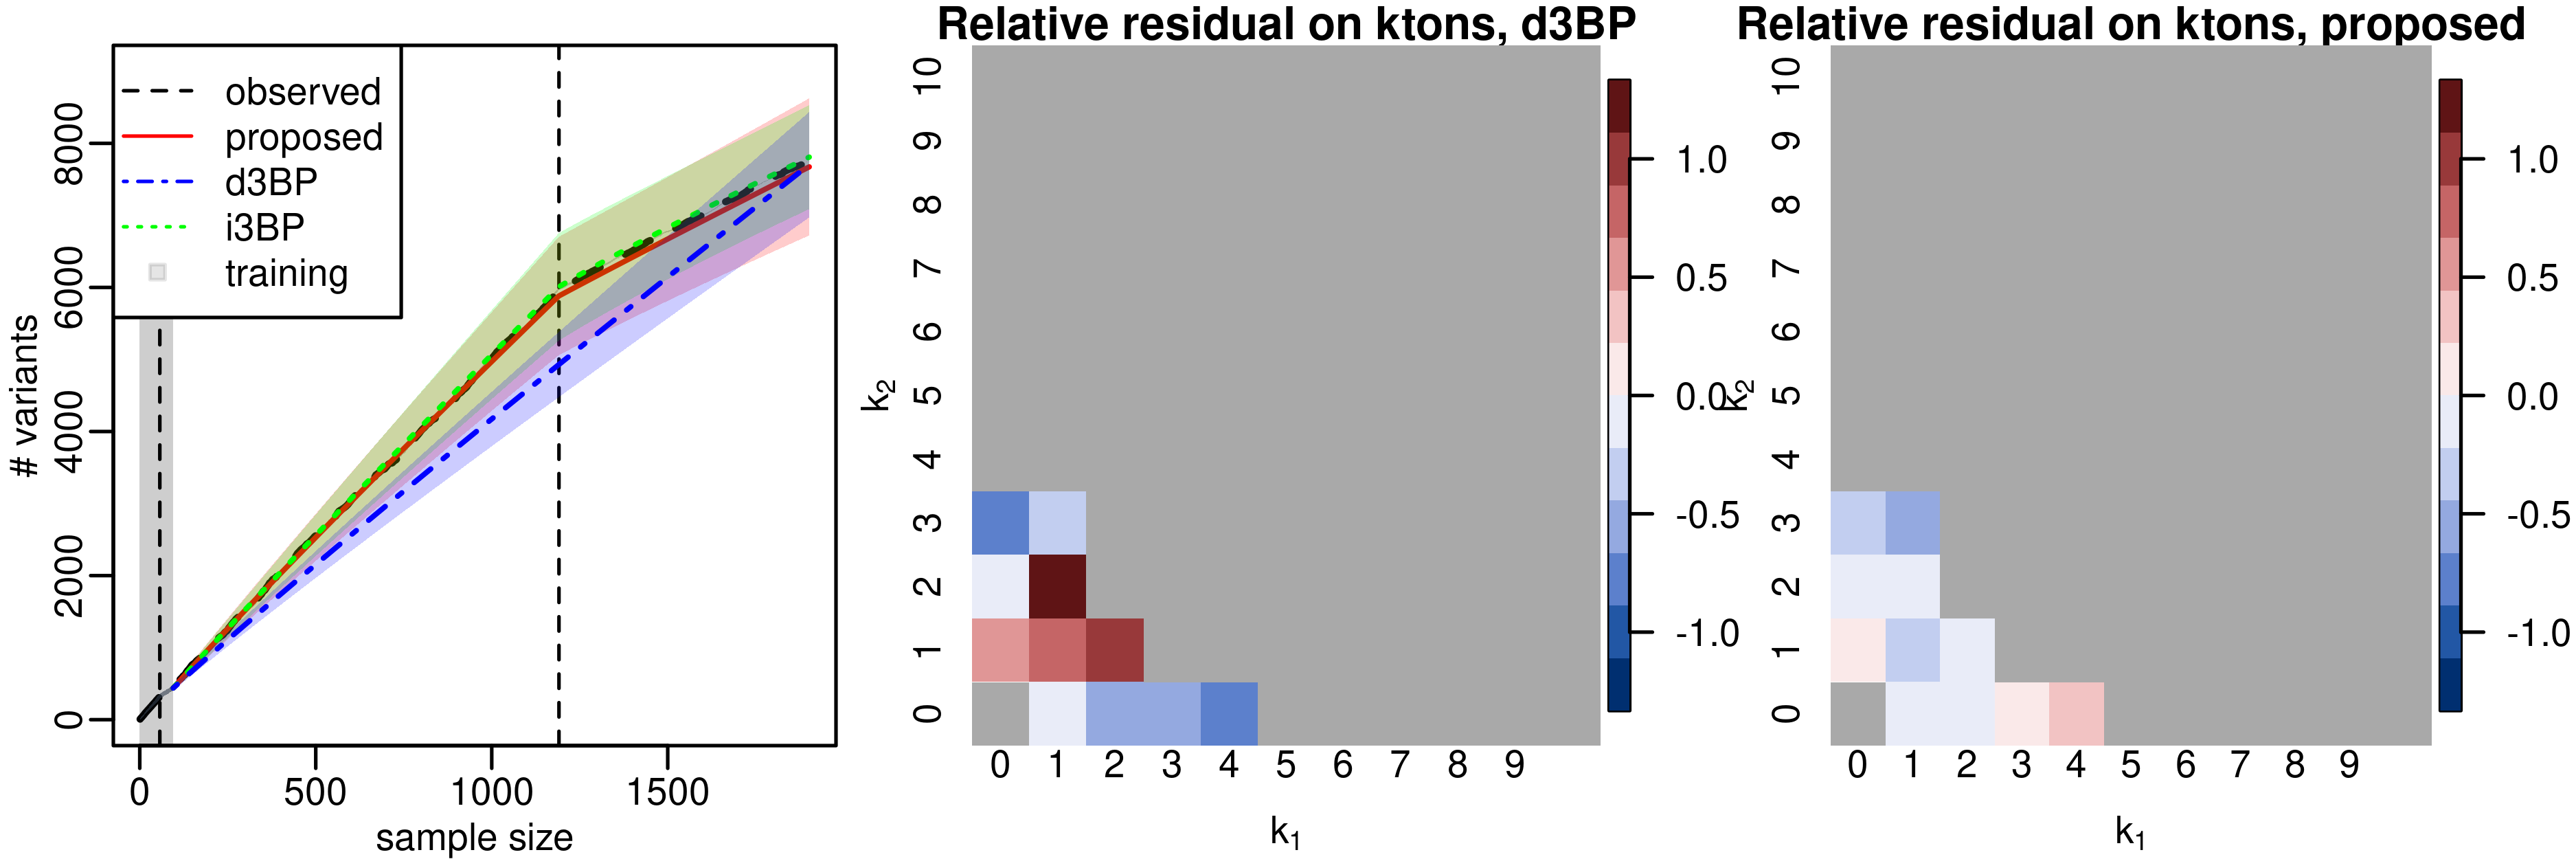
\includegraphics[width = 0.9\textwidth]{Figs/BIDC_LA2_20fold.png}
    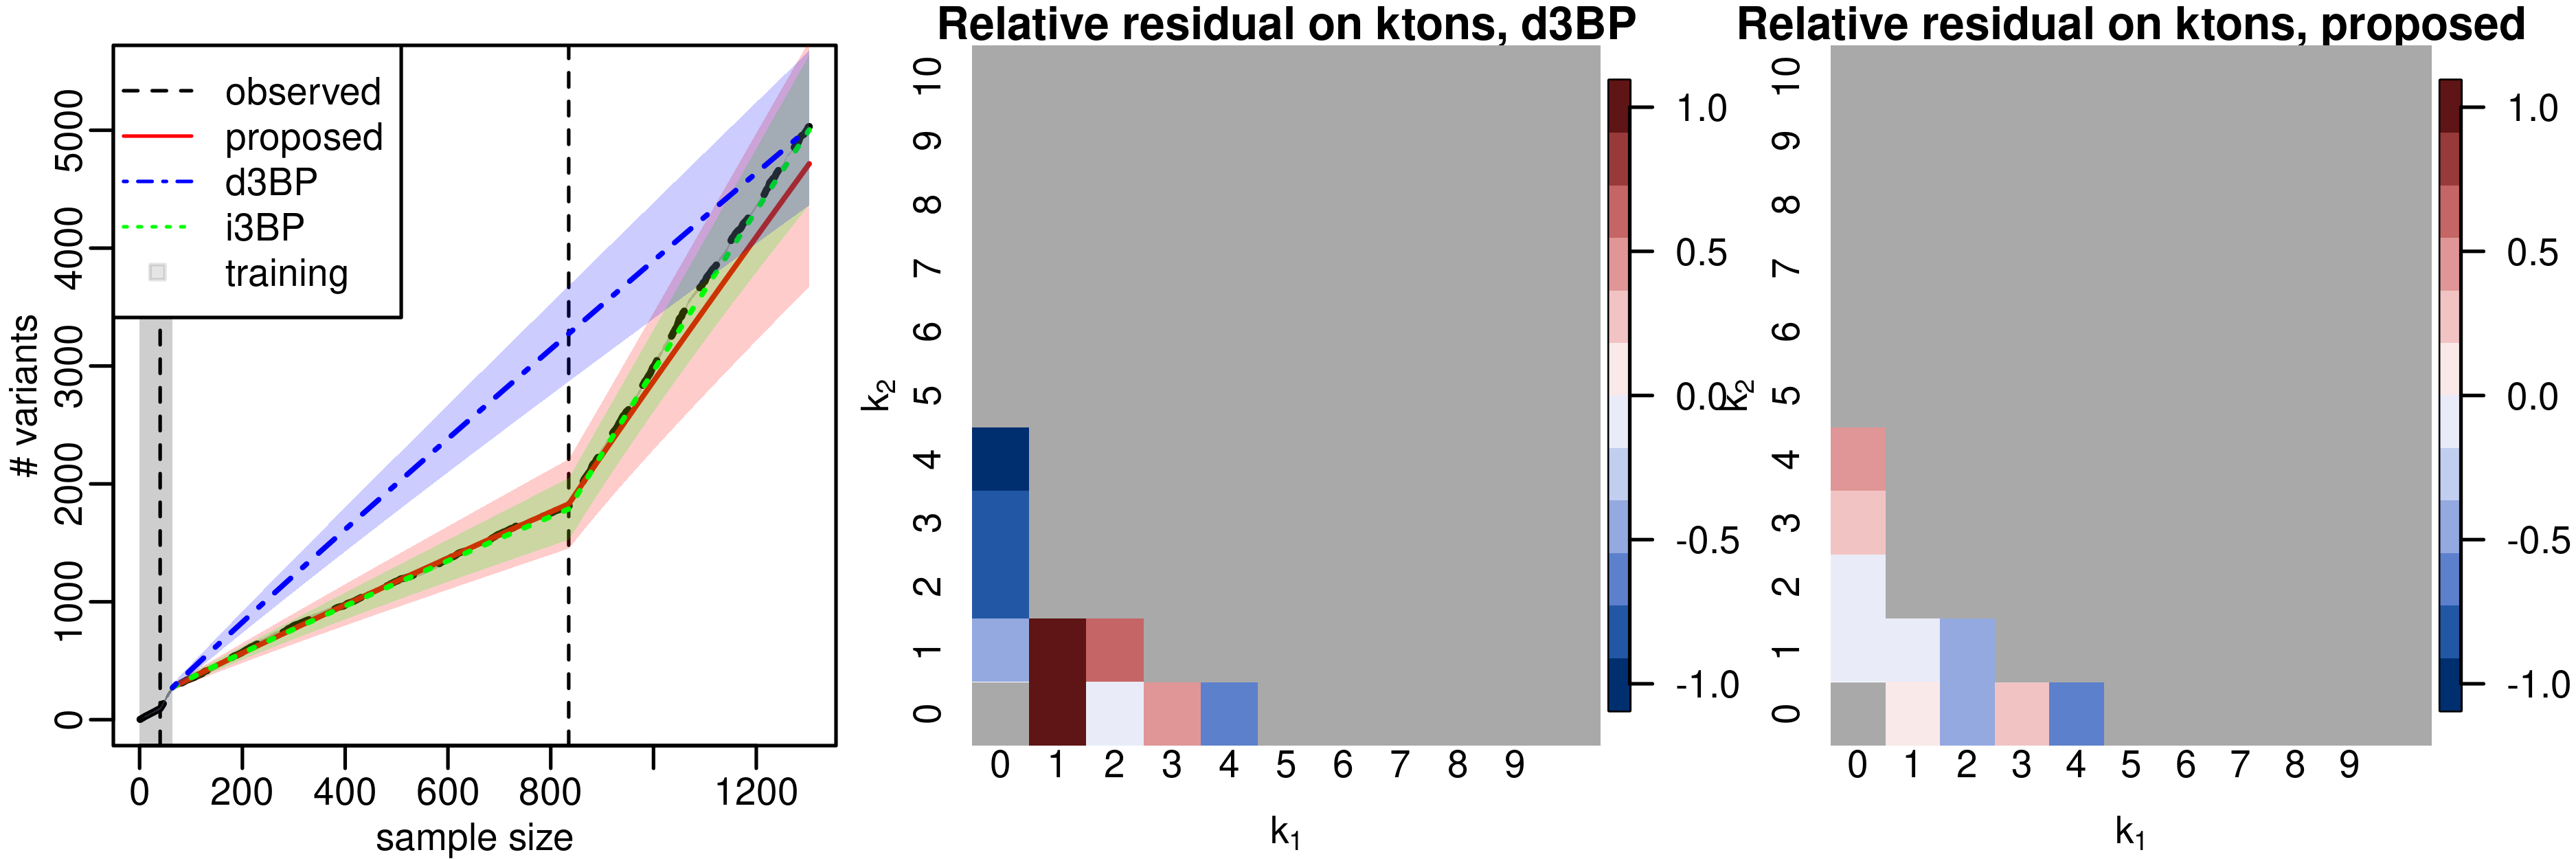
\includegraphics[width = 0.9\textwidth]{Figs/BRCA_LUAD_20fold.png}
    \caption{Predictions for the cancer genomics data. The rows correspond to datasets (upper: MSK-IMPACT, lower: TCGA). Population 1 is breast cancer, and population 2 is lung cancer. Other details of the plots are as in \cref{fig:proposed}.
    }
    \label{fig:cancer}
\end{figure}

The results in \cref{fig:cancer} demonstrate that our method outperforms the two one-population baselines. In particular, both our method and the independent application agree closely with the ground truth number of new variants across the various follow-up sizes (left panels). Indeed, we expect a low level of sharing between cancer types since most variants in cancer are \textit{de novo} variants -- not subject to the natural selection that might make variants more likely to be shared across populations. As expected the dependent application agrees with ground truth when the composition of the follow-up matches the pilot, but its predictions can be very far from the ground truth for other follow-up sizes. In the center and right plots, we see that there are still a number of shared variants with non-trivial counts in the ground truth; see also~Figure S8 of the Supplementary Material \citep{supplement} for direct plots of the ground truth. The independent application is unable to predict such counts. And while the dependent application can predict a non-zero number in these cases, we see from the center and right plots in \cref{fig:cancer} that our method's predictions are more accurate. Overall then, our method is the only one able to provide both useful predictions of the numbers of variants in a follow-up as well as useful predictions of the number of shared variants across populations in the follow-up.


\paragraph{A semi-synthetic population genetics dataset.}
%\label{sec:gnomad}

For population genetics, we use the GnomAD dataset \citep{karczewski2020mutational}. The dataset provides variant frequencies, but it does not provide exact variant data for each sample. So we take the semi-synthetic approach of \citet{Masoero2022}; namely, for each individual, we independently sample the presence of each variant according to the reported frequency of that variant in the data. In general, prediction is more challenging (a) when the pilot is small in absolute terms since less trend information is available 
and (b) when the follow-up is as large as possible since we have a priori more possibility for any observed trend to break down. To accomplish goal (b), we choose large populations: Korean (1909 samples), Bulgarian (1335), and Southern European (5752). We then choose 30 folds to ensure smaller pilots 
(64, 45, and 192, respectively), per goal (a).

For each population (Korean, Bulgarian, Southern European), we compare performance of the one-population \internal{methods listed at the start of} \cref{sec:real_data}; see Section S7.2 of the Supplementary Material \citep{supplement} \internal{for results}. For each population in this case, we find that the fourth-order jackknife (4JK) \internal{is the best performer}. So we use the 4JK for the independent and dependent one-population applications in this analysis.

The results in \cref{fig:pop_gen} demonstrate that our method outperforms the two one-population methods at predicting the number of new variants in a follow-up. When the follow-up composition matches the pilot (the most favorable case for the dependent application), our method is at least on par with the dependent one-population application at predicting the number of shared variants in a follow-up. 
We see in the upper left plot that the dependent application miscounts variants when the composition of the follow-up differs from the pilot. The independent application predicts the first population well but double counts shared variants when the second population appears in the follow-up. In the lower left, the two populations are more similar, so the dependent application performs reasonably; the independent application, though, double counts shared variants in the second population in the follow-up. In both examples, our method tracks closely with ground truth. 

In the upper center plot, we see that the dependent one-population application can be over an order of magnitude off in its predictions. In the upper right plot, we see that our method is much closer to ground truth across the $\vecoccurrence$ values here. Unlike in the cancer data case, the ground truth at all $\vecoccurrence$ values in this plot is substantially greater than zero; see Figure S8 of the Supplementary Material \citep{supplement} for more information about the ground-truth counts. In particular, the signed residual plot in Figure S8 of the Supplementary Material \citep{supplement} shows that the dependent application is providing an overestimate along the diagonal. Indeed, we expect that the Korean and Bulgarian populations have little overlap and thus few shared variants -- whereas the dependent application assumes they are the same population. Conversely, in the lower center and right plots, we see that our method is often farther from the ground truth than the dependent application. We note that the magnitude of the error is smaller than in the upper plots, but it is still quite high (larger than 100\%). It may be that the complex history between the related Southern European and Bulgarian populations cannot be captured by the simple models we consider here.  We reiterate that the independent application predicts zero for all $\vecoccurrence$ values that do not have a zero component and thus fails to predict all such values in these examples.






\begin{figure}[htp]
    \centering
    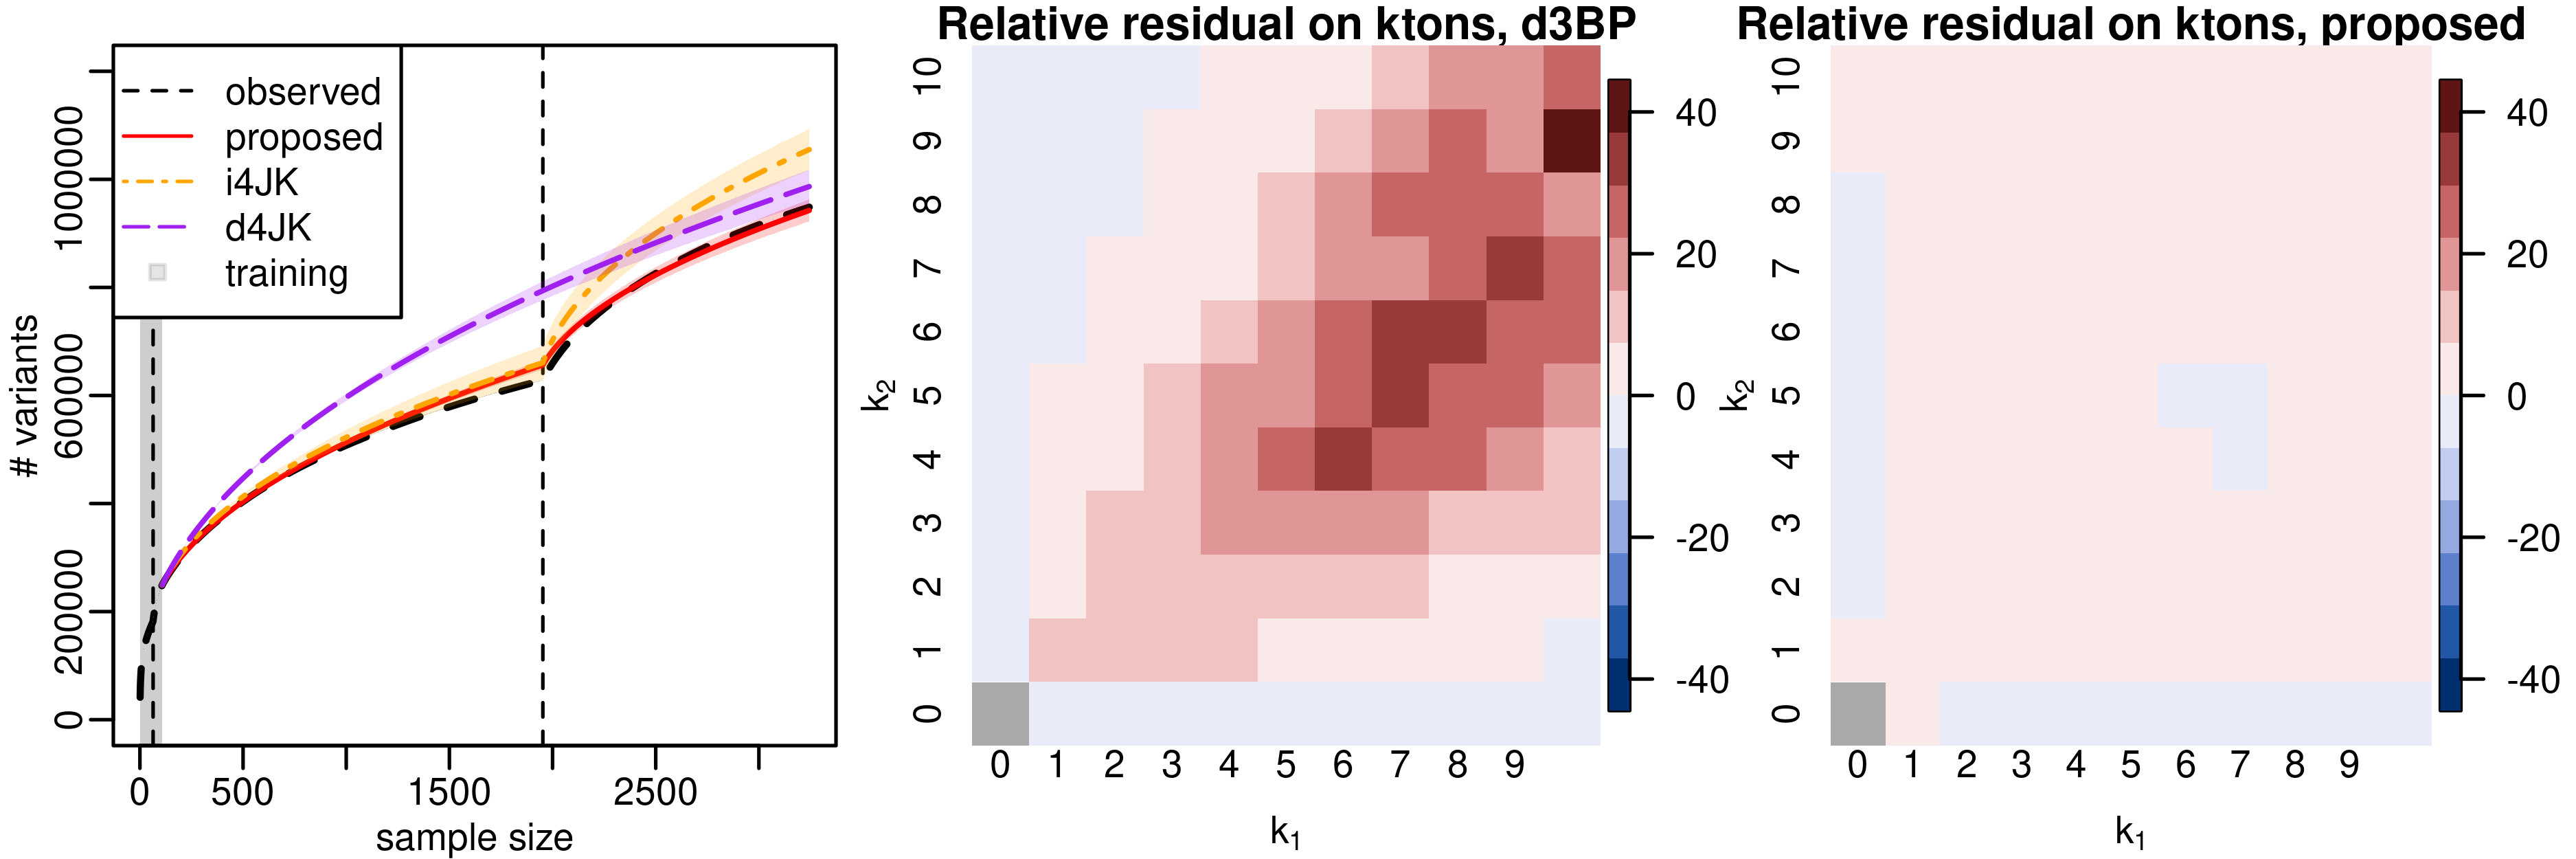
\includegraphics[width = 0.9\textwidth]{Figs/kor_bgr_30fold.png}
    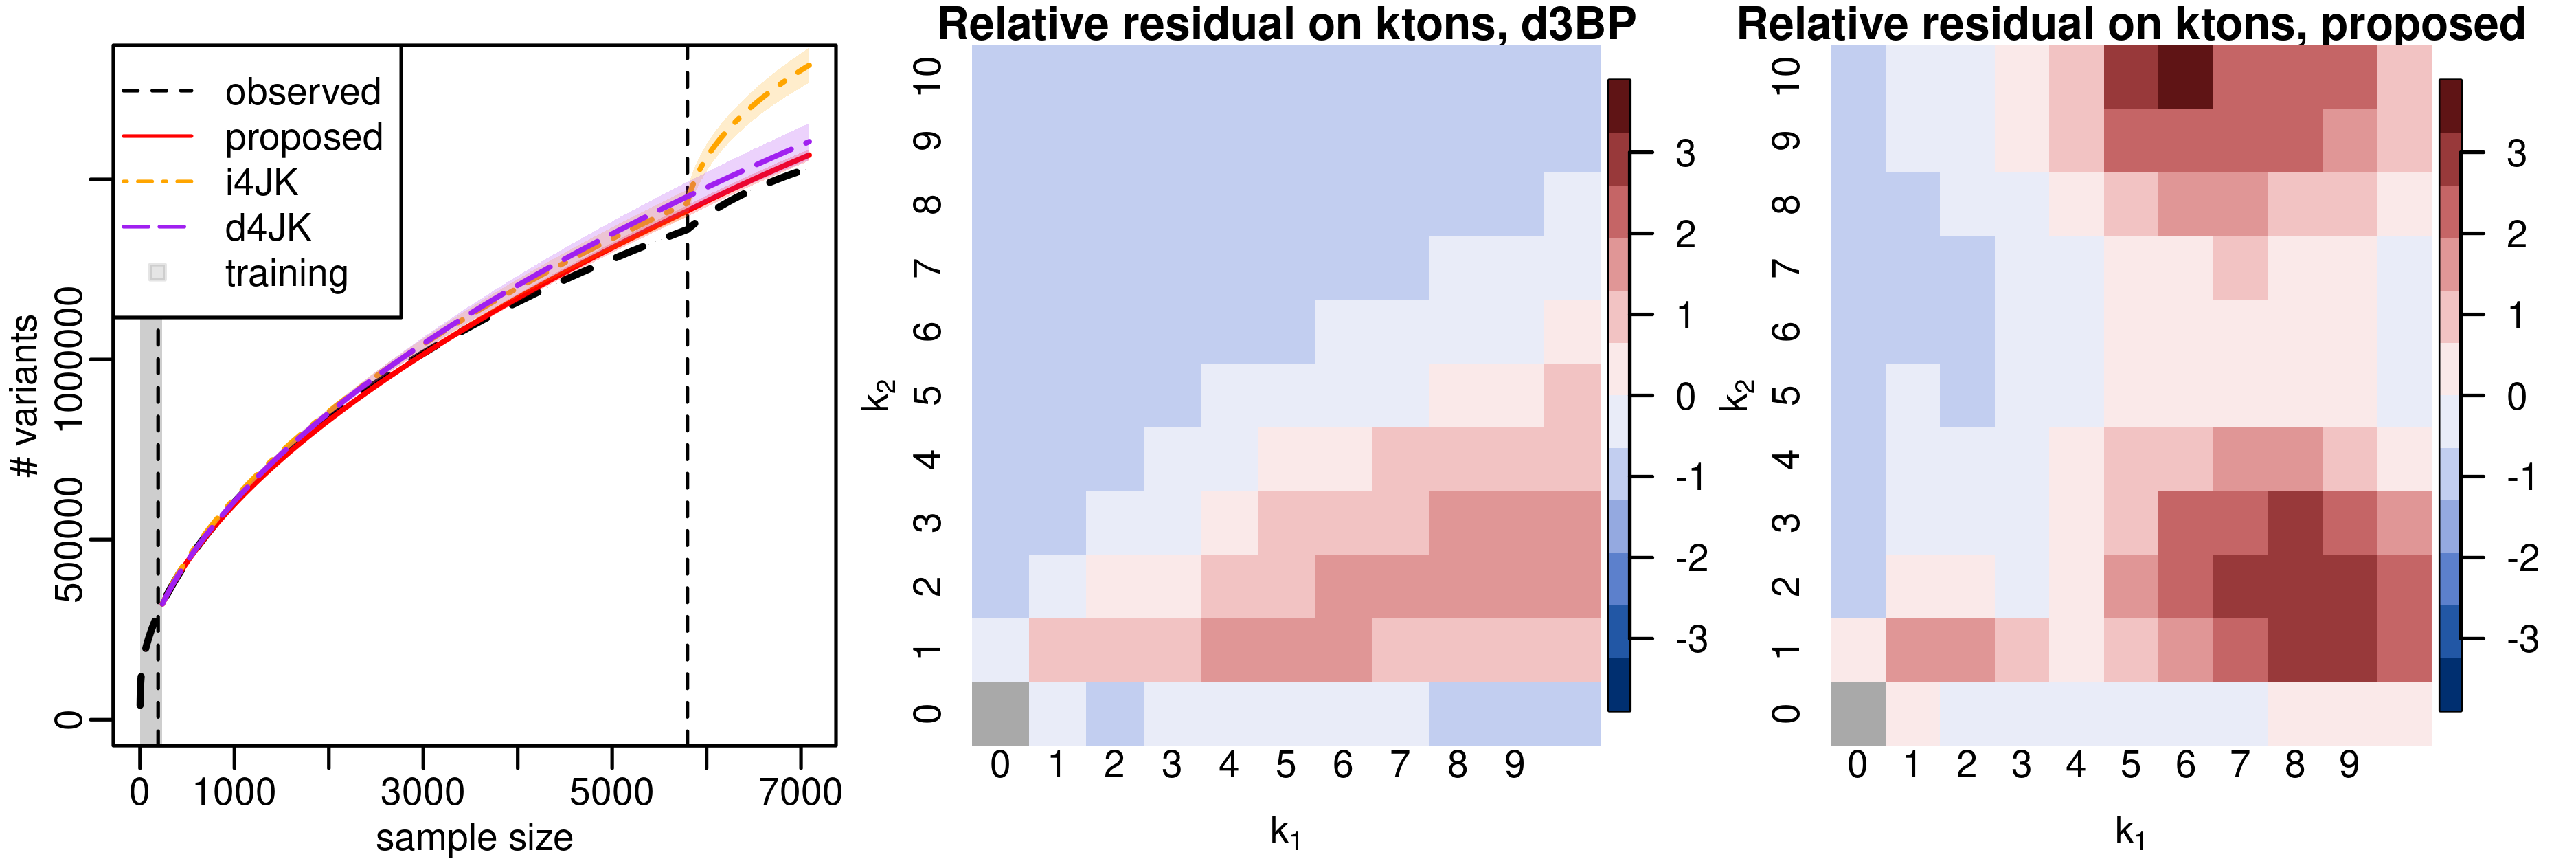
\includegraphics[width = 0.9\textwidth]{Figs/seu_bgr_30fold.png}
    \caption{Predictions for the gnomAD data. The rows correspond to datasets (upper: Korean--Bulgarian, lower: Southern European--Bulgarian). In particular, in the top row, population 1 is Korean, and population 2 is Bulgarian. In the bottom row, population 1 is Southern European, and population 2 is Bulgarian. Other details of the plots are as in \cref{fig:proposed}. We highlight the very different color scales between the upper and lower rows.
    }
   \label{fig:pop_gen}
\end{figure}

